\section{Standard Model of Particle Physics}
The SM is a model based on Quantum Field Theory (QFT) which classifies all known elementary particles and describes their interactions. It is a well-tested model and has shown to be hugely successful in describing experimental data to great precision~\cite{altarelli2014higgs, ALTARELLI_1998}. For example, in the top quark sector, the $t\bar{t}$ cross section predictions have been confirmed to $3.9\%$ accuracy~\cite{cms-ttbar, ATLAS-CONF-2019-041}. It incorporates three of the four fundamental forces of nature: the electromagnetic, the weak and the strong forces. In Figure \ref{fig:SM-particles}, all known elementary particles described by the SM, are shown.

\begin{figure}[h!]
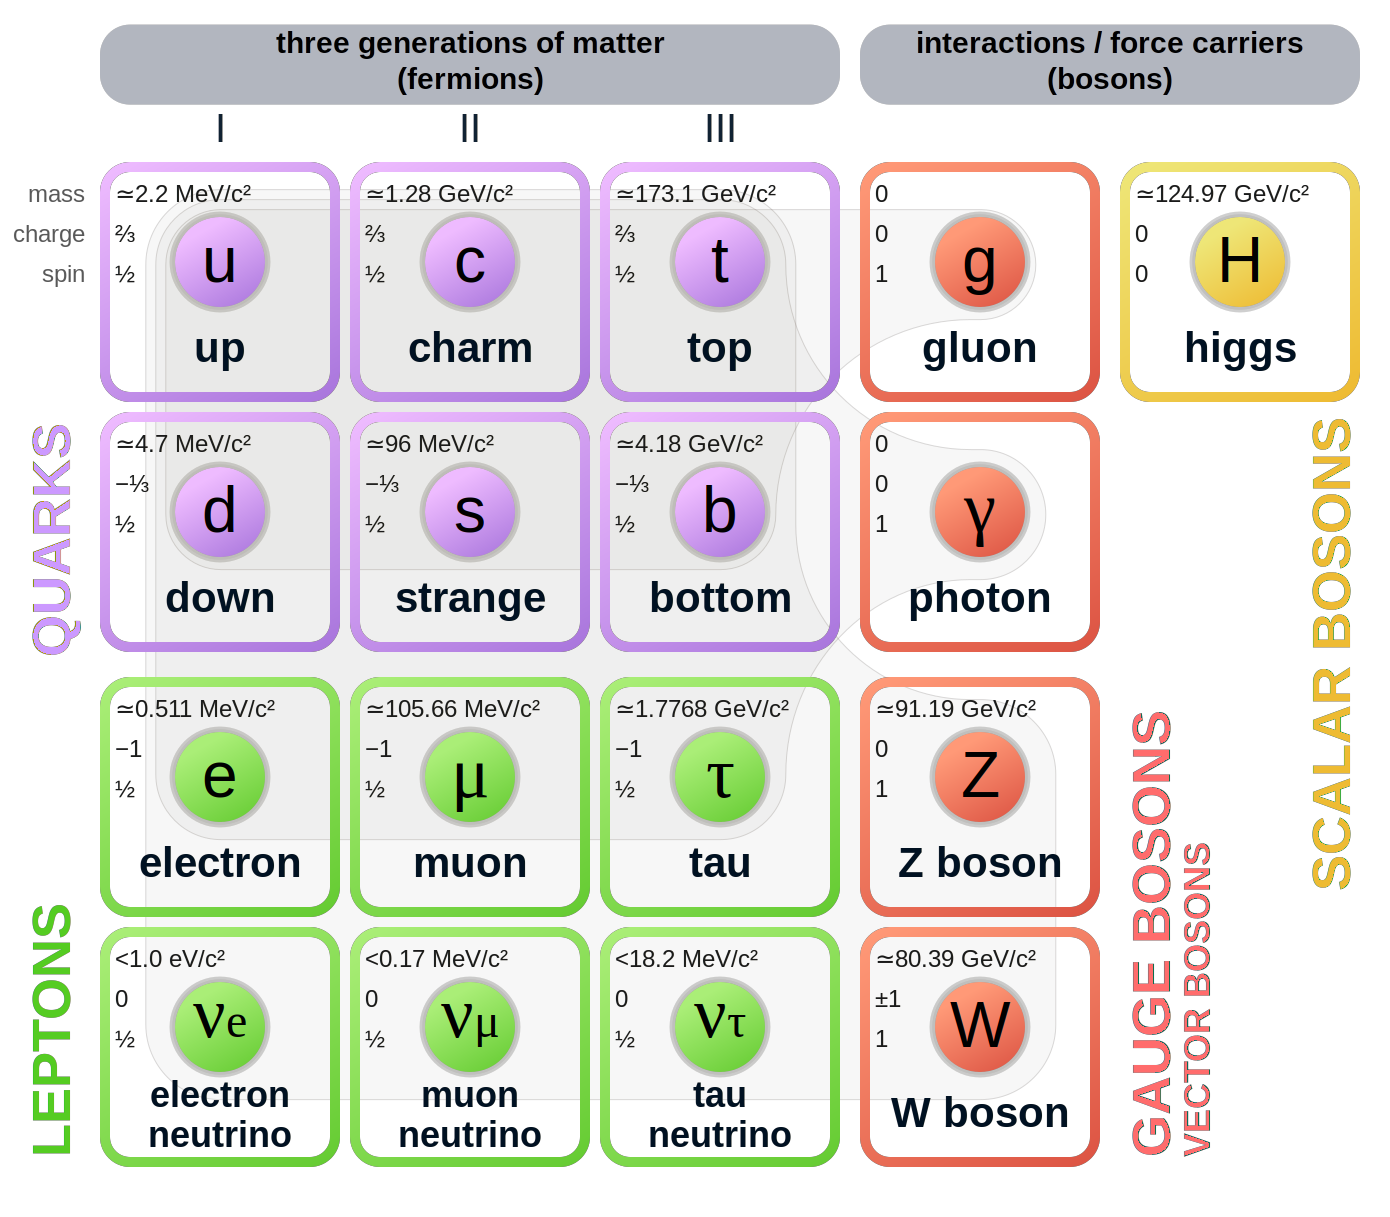
\includegraphics[width=0.6\textwidth]{figures/theoryFigs/SM_particles.png}
\centering
\caption{A summary of the elementary particles described by the SM~\cite{SM-picture} is shown. Fermions are shown on the left, with quarks shown in purple and leptons shown in green. Bosons are shown on the right, with gauge bosons shown in red and the Higgs boson shown in yellow. The mass, electric charge and spin of each particle is shown on the top left of each particle's block.}
\label{fig:SM-particles}
\end{figure}
\noindent
Particles in the SM are uniquely described by their quantum numbers: electric charge and spin. The SM particles are split into main two classes, based off their spin quantum numbers. Particles which have half-integer spin are called fermions, and those which have integer spin are called bosons. Fermions are further divided into three generations, each comprising of two quarks, one charged lepton and one neutrino. In a generation, the more massive quark has an electric charge of $+2/3$ (up-type) and the less massive quark has an electric charge of $-1/3$ (down-type). All charged leptons have an electric charge of $-1$ and all neutrinos are electrically neutral. The masses of the particles in a generation increase with increasing generation number, with generation 1 particles being the least massive and generation 3 particles being the most massive. Quarks carry electric and colour charge, and can therefore interact via the electromagnetic, weak and strong forces. Colour charge can take on three values: red, green and blue. It is important to note that colour charge is completely unrelated to the everyday meaning of colour, and it just represents the quantum state of the particle. Due to colour confinement~\cite{quark-confinement}, quarks cannot be isolated from one another. They exist in colourless bound states, called hadrons, consisting of two or more quarks. Hadrons consisting of an even number of quarks are known as mesons and those consisting of an odd number of quarks are known as baryons. On the other hand, charged leptons (electron ($e$), muon ($\mu$) and tau ($\tau$)) only carry electric charge and can therefore interact electromagnetically and weakly, but not through the strong interaction. The electric and colour neutral fermions, neutrinos, can only interact via the weak force.\\

\noindent
Particles are able to interact with one-another via the exchange of a gauge boson (boson with spin-1). Photons are massless, spin-1 gauge bosons which mediate electromagnetic interactions between particles which carry electric charge, such as quarks and charged leptons ($e$, $\mu$ and $\tau$). The weak interaction is mediated by three massive gauge bosons, the electrically charged $W^{+}$ and $W^{-}$ bosons and the electrically neutral $Z$ boson. Gluons are massless, spin-1 gauge bosons which mediate strong interactions between particles which carry colour charge, such as quarks. Since gluons carry colour charge, they interact with themselves. The massive, spin-0, electrically neutral Higgs boson mediates the Higgs field which gives mass to the $W^{\pm}$ and $Z$ bosons via the so-called Brout-Englert-Higgs mechanism~\cite{PhysRevLett.13.321, Higgs:1966ev, Higgs:1964pj}. The Brout-Englert-Higgs mechanism induces spontaneous electroweak symmetry breaking to provide mass terms for the $W^{\pm}$ and $Z$ bosons in the electroweak Lagrangian of the SM. All particles described in the SM have their own antiparticle, with the same mass, but opposite charges. Some particles, such as the photon, are their own antiparticle.\\

\noindent
Although the SM has shown to be hugely successful, it is incomplete and fails to describe certain observed phenomena. The most notable example being the absence of gravity from the SM. The gravitational force is $\approx 10^{29}$~\cite{thomson2013modern} weaker than the weak force, therefore quantum gravitational effects are expected to only become significant at energies much larger than that currently accessible by the LHC (known as the Planck scale $\approx 10^{9}$ GeV)~\cite{hierarchy-problem-paper}. This large difference in strength between the weak force and gravity is known as the Hierarchy Problem. Cosmological observations infer that around 84$\%$ of the matter in the universe consists of gravitationally interacting matter known as dark matter~\cite{Jarosik_2011}. None of the particles described in the SM are good dark matter candidates, therefore the SM only accounts for a small fraction of the total matter of the universe. The large discrepancy between the observed amount of matter and antimatter in the universe, sometimes referred to as the matter-antimatter asymmetry, is not fully explained by the SM. Neutrinos in the SM are assumed to be massless, however observations of neutrino oscillations (neutrinos undergoing flavour change as they travel through space) imply that neutrinos do have mass~\cite{fantini2020formalism}. Beyond the Standard Model (BSM) theories attempt to explain the phenomena which the SM cannot. For example, a popular extension to the SM, Supersymmetry (SUSY) introduces new particles to the SM which are counterparts to the existing SM particles with the same quantum numbers, except for their spins~\cite{kirsten2010introduction}. SUSY provides elegant explanations to many shortcomings of the SM, however none of the supersymmetric particles described by SUSY have been observed experimentally~\cite{CANEPA2019100033}.

\subsection{The Top Quark}
The top quark is the heaviest particle in the SM, with a mass of 172.76 $\pm$ 0.30 GeV~\cite{pdg}. According to the SM, since the coupling to the Higgs boson is proportional to the the mass of the interacting particle, the top quark is strongly coupled to the Higgs boson. Physics processes involving top quarks is therefore a theoretically well-motivated area to search for new physics, since it is the most likely particle to couple to new physics theories at the TeV scale. Its large mass also makes it highly unstable, with a mean lifetime of $\approx 0.5 \times 10^{-24}$ s~\cite{pdg}. The top quark's lifetime is shorter than that of the hadronisation process, and it therefore decays before hadronising. The top quark can therefore be measured indirectly via its decay products. Top quarks almost always decay to a $W$ boson and a $b$-quark ($\frac{\Gamma(Wb)}{\Gamma( Wq (q=b,s,d))} = 0.957\pm 0.034$~\cite{pdg}). The $b$-quark is the second heaviest quark in the SM, however its lifetime is still longer than the hadronisation time scale~\cite{pdg}. In hadron collider experiments, $b$-quarks travel a short distance in the detector before hadronising to form jets. In Table \ref{tab:top-decay-modes}, the dominant final state branching fractions of the top quark are shown.

\begin{table}[h!]
\def\arraystretch{1.5}%
\begin{tabular}{l|c}
\hline
Decay Mode & Branching Fraction ($\frac{\Gamma_{i}}{\Gamma}$)\\ \hline
$t \rightarrow Wb \rightarrow e\nu_{e} b$           &      $(11.10\pm 0.30)\%$     \\
$t \rightarrow Wb \rightarrow \mu \nu_{\mu} b$             &   $(11.40\pm 0.20)\%$        \\
       $t \rightarrow Wb \rightarrow \tau \nu_{\tau} b$      &  $(10.70\pm 0.50)\%$         \\
  $t \rightarrow Wb\rightarrow q\bar{q} b$           &      $(66.50\pm 1.40)\%$     \\ \hline
\end{tabular}
\centering
\caption{The dominant final state branching fractions of the top quark~\cite{pdg} are shown.}
\label{tab:top-decay-modes}
\end{table}

\noindent
Hadronic final states are more than twice as likely than leptonic final states. Final state decays to different lepton flavours are roughly equally probable.\\

\noindent
Top quark production can be placed into two main categories: pair production ($t\bar{t}$) and single-top production ($t$)~\cite{dasilva2016quark}. In the LHC, top quarks are mainly produced in pairs via strong interactions in gluon-gluon fusion ($gg\rightarrow t\bar{t}$) or quark annihilation ($q\bar{q}\rightarrow t\bar{t}$). Top quark production via gluon-gluon fusion is the dominating process~\cite{Ball_2015}. The production cross section for $t\bar{t}$ (leptonic final state) in $pp$ collisions with $\sqrt{s} = 13$ TeV was measured by ATLAS with a value of $830 \pm 0.4 (\text{stat}) \pm 36 (\text{syst}) \pm 14 (\text{lumi})$ pb~\cite{ATLAS-tt-crossSection-2020}, with good agreement between measurement and theoretical prediction.\\

\noindent
Single top production occurs via the weak interaction. The most abundant production mechanisms leading to single top production are the $s$-, $t$- and $Wt$- channels~\cite{pdg}. In the $s$-channel, an initial quark annihilates with an anti-quark of different flavour, producing a virtual $W$ boson which decays to a top quark and anti-bottom quark. In the $t$-channel, an initial $b$ quark interacts with a different flavour quark via the exchange of a $W$ boson. This interaction produces a top quark and another quark. In the $Wt$-channel, an initial gluon interacts with a $b$ quark to produce a top quark and a $W$ boson, either via the absorption of the gluon by the $b$ quark or via the exchange of a top quark. In Table \ref{tab:single-top-crossSection}, single top production cross sections in $pp$ collisions at $\sqrt{s}=13$ TeV for the $s$-, $t$- and $Wt$-channels, are shown.


\begin{table}[h!]
\def\arraystretch{1.5}%
\begin{tabular}{c|c|c}
\hline
Channel & Process & Total Cross Section [pb] \\ \hline
$s$& $q\bar{q'}\rightarrow   W \rightarrow \bar{b}t$& $10.32^{+0.40}_{-0.36}$  \\
$t$ & $bq'\rightarrow W \rightarrow tq$ &  $216.99^{+9.04}_{-7.71}$\\
$Wt$& $bg \rightarrow  b/t \rightarrow Wt$ &  $71.7\pm 3.85$\\ \hline
\end{tabular}
\centering
\caption{Single top production cross sections in $pp$ collisions at $\sqrt{s}=13$ TeV for the $s$-, $t$- and $Wt$-channels~\cite{summaryPlots} are shown. The prime superscript on $q^{'}$ indicates that the quark has a different flavour to $q$. }
\label{tab:single-top-crossSection}
\end{table}
\noindent
Single top production is suppressed compared to pair produced top production, with $t\bar{t}$ production (leptonic final state) being around three times as likely to occur than single top production across all decay channels.


\subsubsection{Motivation for the search for $tWZ$ production in the tetralepton channel}
The recent lack of signs of new physics from LHC data~\cite{sonneveld2019searches} tells us that new physics is either very heavy, or is very weakly coupled to SM particles. We therefore might only observe signs of new physics in anomalous rates of well-chosen processes. The $tWZ$ process is a prime example of such a process. It has an extremely low production cross section (0.7 fb for $\sqrt{s}= 13$ TeV~\cite{twz-theory-paper}), and has subsequently never been observed by any particle physics experiment. Since $tWZ$ involves a charged $W$ boson and neutral $Z$ boson, its cross section is sensitive to the charged and neutral couplings to the top quark. In turn, the top quark is strongly coupled to the Higgs boson, due to its large mass. Due to the top quark's large coupling to the Higgs boson, corrections to the Higgs boson mass diverge in the SM. The top quark's couplings are modified, in order to remove this divergence, in many scenarios of new physics that aim to resolve the Hierarchy Problem. Since the $Z$ boson may be radiated from the initial-state $b$-quark, the final-state top quark, or the final-state $Z$ boson, the $tWZ$ process embeds the $b-Z$, $t-Z$ and $W-Z$ electroweak couplings which are often modified in BSM physics. Therefore $tWZ$ is an important process in the search for signs of new physics and BSM physics.\\ %\cite{Chaichian_1995}???

\noindent
One such BSM theory which is sensitive to $tWZ$ production~\cite{Maltoni_2019, mimasu2021quark} is the Standard Model Effective Field Theory (SMEFT)~\cite{Brivio_2019}. The SMEFT attempts to describe physics at large energy scales which we have not yet been able to probe experimentally. The SMEFT inherits the same QFT framework as the SM, and adds Lagrangian terms to the SM Lagrangian which describe the interactions of SM particles at higher energy scales. Analogous to the coupling constants found in the SM Lagrangian, which indicate the interaction strengths between different particles, SMEFT contains scalar coefficients which operate in the same way. These scalar coefficients are known as Wilson coefficients. It has been shown that the cross section of $tWZ$ is sensitive to many Wilson coefficients. An experimental constraint on the cross section of $tWZ$ is therefore expected to be impactful on a global fit on all the Wilson coefficients in SMEFT.\\

\noindent
Prior to this analysis, only three experimental studies of $tWZ$ in ATLAS have been performed. The first and third studies utilised the trilepton channel to search for $tWZ$ production, whereas the second study utilised both the tri- and tetralepton channels. The first search utilised 36 fb$^{-1}$ of ATLAS data and an upper limit on the cross section of $tWZ$ was set at a value of $\approx$ 6 times the SM cross section~\cite{twz_3_lep}. The second study investigated the feasibility of a cross section measurement of $tWZ$ production with CMS Run 3 data (300 fb$^{-1}$)~\cite{Tschida:2020ftz}. The study showed that it is possible to exclude $\mu (tWZ)$ at the $7\sigma$ significance level using 300 fb$^{-1}$ of data. This study needs to be further investigated, since its findings seem improbable given the results obtained in this thesis. The third search utilised 139 $^{-1}$ of ATLAS data and an expected upper limit on the cross section of $tWZ$ was set at a value of $\approx$ 2.6 times the SM cross section~\cite{ben-thesis}. In Section \ref{sec:combined-results}, the latter analysis will be used in combination with this analysis, in order to further increase the sensitivity of the cross section of $tWZ$.



%\section{Effective Field Theory (EFT)}
%Brief overview of EFT. What is EFT? Why important to pp as a whole? Why important in twz (high sensitivity to wilson coefficients, expected to have a large impact on global fit)? Similar to what james says in INT note.
%\section{Machine Learning in the Context of Particle Physics Analyses}
%Brief overview of ML as a whole; History; increase in popularity in recent years (why increased in popularity $\rightarrow$ novel techniques developed, increase in computing power for your buck). Where does it fit into pp (event selection, object reconstruction and ID (jet reco, b-tagging)). Explain concepts (vocabulary), overtraining, training, testing, classifier, classification. Why use x train/test ratio in pp (use some for analysis/use some for training)? Popular tools which are used today (scikit learn, TMVA, xgboost what is theano, what is keras).\\
%Maybe a subsection on bdt (if end up using it) on the specific algorithm, and minimizing cost function (general). Explanation on ROC curve and why we can use it as a proxy to determine how well our bdt/nn is doing (and where it fails/can fail $\rightarrow$ things to be aware of cautious of when straight up using ROC integral (e.g. overtraining )).
%\section{Statistical Techniques}
%Brief overview: frequentist and bayes approach in general in pp, why we use frequentist in this analysis



\section{$tWZ$}
\subsection{Tetralepton Channel}
In Figure \ref{fig:twzfourlep_FeymanDiagram}, the Leading Order (LO) Feynman diagram for \tWZ in the tetralepton channel, is shown.

\begin{figure}[h!]
	
\centering
\begin{tikzpicture}[thick,scale=0.6, every node/.style={transform shape}]

\begin{feynman}
\vertex (a) {$b$};
\vertex [below right=of a] (c);
\vertex [below left=of c] (b) {$g$};

\vertex [right=of c] (d);  %d: tW vertex

\vertex [above right=3cm of d] (e);  %e: top vertex

\vertex [below right=3cm of e] (i);  %i: Z -> ll vertex
\vertex [above right=of i] (f1) {$\ell^{\mp}$}; 
\vertex [below right=of i] (f2) {$\ell^{\pm}$}; 


\vertex [above right=2cm of e] (f);  %f: Wb vertex
\vertex [below right=of f] (f7) {$b$};

\vertex [above right=of f] (g);  %g: l \nu vertex
\vertex [below right=of g] (f3) {${\nu}_{\ell}$};
\vertex [above right=of g] (f4) {$\ell^{+}$};


\vertex  [below right=6cm of d] (h); %h: l \nu vertex (bottom)
\vertex [below right=of h] (f5) {$\bar{\nu}_{\ell}$};
\vertex [above right=of h] (f6) {$\ell^{-}$};



\diagram* {
	(a) -- [fermion] (c),
	(b) -- [gluon] (c),
	(c) -- [fermion, edge label=$b$] (d),
	(d) -- [fermion, edge label=$t$] (e),
	
	(e) -- [boson, edge label=$Z$] (i),
	(i) -- [fermion] (f1),
	(i) -- [anti fermion] (f2),
	
	(f) -- [boson, edge label=$W^{+}$] (g),
	(e) -- [fermion] (f),
	(f) -- [fermion] (f7),
	(g) -- [fermion] (f3),
	(g) -- [anti fermion] (f4),
	

	
	(d) -- [boson, edge label=$W^{-}$] (h),
 	(h) -- [anti fermion] (f5),
	(h) -- [fermion] (f6),
	
	
};
\end{feynman}

\end{tikzpicture}
\caption{The LO Feynman diagram of \tWZ production in the tetralepton channel is shown.}
\label{fig:twzfourlep_FeymanDiagram}
\end{figure}



\subsubsection{Backgrounds}
The main backgrounds for \tWZ (tetralepton channel) are the production of a two tops, both in the $\ell \nu b$~\footnote{In this thesis, $\ell$ refers to an electron or muon, $\nu$ refers to a neutrino or anti-neutrino and $b$ refers to a bottom quark or anti-bottom quark} final state channel, together with a $Z$ boson (\ttZ) and diboson production with fully leptonic final states (\ZZ). In Figure \ref{fig:ttz_and_zz_feynman}, LO Feynman diagrams for \ttZ and \ZZ in the tetralepton channel, are shown.

\begin{minipage}{.5\textwidth}
	\centering
\begin{tikzpicture}[thick,scale=0.6, every node/.style={transform shape}]


\begin{feynman}

\vertex (a) {$g$};
\vertex [below right=of a] (c);
\vertex [below left=of c] (b) {$g$};

\vertex [right=of c] (d);   %g -> ttbar vertex

\vertex [above right=3cm of d] (e);   %d: t-> Wb vertex
\vertex [below right=3cm of d] (f);   %e: t bar-> Z tbar vertex

%t-> Wb vertex
\vertex [above right=3cm of e] (g);  %(g): W-> l\nu (top)
\vertex [above right=of g] (f1)  {$\ell^{+}$};  
\vertex [below right=of g] (f2)  {$\nu_{\ell}$}; 
\vertex [below right=of e] (f3)  {$b$};   

\vertex [above right=3cm of f] (h);   %(h): Z-> ll vertex 
\vertex [above right=of h] (f4) {$\ell^{\mp}$}; 
\vertex [below right=of h] (f5)  {$\ell^{\pm}$}; 


\vertex [below right=2cm of f] (i);   %(i): tbar-> bW
\vertex [above right=of i] (f6)  {$\bar{b}$};  
\vertex [below right=2cm of i] (j);   %W-> l\nu vertex (tbar)
\vertex [above right=of j] (f7)  {$\ell^{-}$};  
\vertex [below right=of j] (f8)  {$\bar{\nu}_{\ell}$}; 





\diagram* {
	
	(a) -- [gluon] (c),
	(b) -- [gluon] (c),
	
	(c) -- [gluon, edge label=$g$] (d),
	
	(d) -- [fermion, edge label =$t$](e),
	(d) -- [anti fermion, edge label'=$\bar{t}$](f),
	
	(e) -- [boson, edge label=$W^{+}$] (g),
	(e) -- [fermion] (f3),
	(g) -- [anti fermion] (f1),
	(g) -- [fermion] (f2),
	
	(f) -- [boson, edge label=$Z$] (h),
	(h) -- [fermion] (f4),
	(h) -- [fermion] (f5),
	
	(f) -- [anti fermion] (i),
	(i) -- [anti fermion] (f6),
	(i) -- [boson, edge label=$W^{-}$] (j),
	(j) -- [fermion] (f7),
	(j) -- [anti fermion] (f8),
	
	
	
	
	
};
\end{feynman}
\end{tikzpicture}
\end{minipage}% This must go next to `\end{minipage}`
\begin{minipage}{.5\textwidth}
	\centering
	\begin{tikzpicture}[thick,scale=0.6, every node/.style={transform shape}]
	\label{fig:zz_FeymanDiagram}
	
	\begin{feynman}
	
	\vertex (a) {$q$};
	\vertex [below right=of a] (c);
	\vertex [below left=of c] (b) {$\bar{q}$};
	
	\vertex [above right=3cm of d] (e); % Z vertex (top)
	\vertex [above right=of e] (f1) {$\ell^{\mp}$}; 
	\vertex [below right=of e] (f2) {$\ell^{\pm}$}; 
	
	
	\vertex [below right=3cm of d] (f); % Z vertex (bottom)
	\vertex [above right=of f] (f3) {$\ell^{\mp}$}; 
	\vertex [below right=of f] (f4) {$\ell^{\pm}$}; 
	
	
	
	
	\diagram* {
		
		(a) -- [fermion] (c),
		(b) -- [anti fermion] (c),
		
		(c) -- [boson, edge label=$Z/ \gamma$] (d),
		
		(d) -- [boson, edge label=$Z$] (e),
		(d) -- [boson, edge label=$Z$] (f),
		
		(e) -- [fermion] (f1),
		(e) -- [anti fermion] (f2),
		
		(f) -- [fermion] (f3),
		(f) -- [anti fermion] (f4)
		
			
	};
	\end{feynman}
	\end{tikzpicture}

\end{minipage}
\label{fig:ttz_and_zz_feynman}
\captionof{figure}{LO Feynman diagrams for \ttZ (left) and \ZZ (right) in the tetralepton channel are shown.}
\vspace{1cm}
The $t\bar{t}Z$ process contains fours leptons and two $b$-quarks in its final state (inclusive $\sigma(t\bar{t}Z)= 0.95 \pm 0.08_{\text{stat}} \pm 0.10_{syst}$ pb at $\sqrt{s}=13$ TeV~\cite{ttz-xsec-paper}) and can easily mimic the \tWZ signal process, for instance, by one of its $b$-jets getting missed during detection. The \ZZ process contains four leptons and zero $b$-quarks in its final state (inclusive $\sigma(ZZ)= 14.6^{+1.9}_{-1.8}(\text{stat})^{+0.5}_{-0.3}(\text{syst})\pm 0.2 (\text{theo})\pm 0.4 (\text{lumi})$ pb at $\sqrt{s}=13$ TeV~\cite{zz-xsec-paper}). One way in which \ZZ can mimic the \tWZ signal process is by reconstruction of a non-prompt $b$-jet. 



\subsection{Comparison to Trilepton Channel}

%Less backgrounds to deal with (in tetralepton). However lower stats (in tetra). Give cross sections (and feynman diagram). Maybe talk a bit about analysis related challenges (trilepton has a hadronically decaying W, does this make the analysis easier or more difficult?).


\begin{figure}[h!]
	
	\centering
	\begin{tikzpicture}[thick,scale=0.6, every node/.style={transform shape}]
	\label{fig:twz3lep_FeymanDiagram}
	\begin{feynman}
	\vertex (a) {$b$};
	\vertex [below right=of a] (c);
	\vertex [below left=of c] (b) {$g$};
	
	\vertex [right=of c] (d);  %d: tW vertex
	
	\vertex [above right=3cm of d] (e);  %e: top vertex
	
	\vertex [below right=3cm of e] (i);  %i: Z -> ll vertex
	\vertex [above right=of i] (f1) {$\ell^{\mp}$}; 
	\vertex [below right=of i] (f2) {$\ell^{\pm}$}; 
	
	
	\vertex [above right=2cm of e] (f);  %f: Wb vertex
	\vertex [below right=of f] (f7) {$b$};
	
	\vertex [above right=of f] (g);  %g: l \nu vertex
	\vertex [below right=of g] (f3) {${\nu}_{\ell}, q$};
	\vertex [above right=of g] (f4) {$\ell^{+}, \bar{q}$};
	
	
	\vertex  [below right=6cm of d] (h); %h: l \nu vertex (bottom)
	\vertex [below right=of h] (f5) {$\bar{q}, \bar{\nu}_{\ell}$};
	\vertex [above right=of h] (f6) {$q, \ell^{-}$};
	
	
	
	\diagram* {
		(a) -- [fermion] (c),
		(b) -- [gluon] (c),
		(c) -- [fermion, edge label=$b$] (d),
		(d) -- [fermion, edge label=$t$] (e),
		
		(e) -- [boson, edge label=$Z$] (i),
		(i) -- [fermion] (f1),
		(i) -- [anti fermion] (f2),
		
		(f) -- [boson, edge label=$W^{+}$] (g),
		(e) -- [fermion] (f),
		(f) -- [fermion] (f7),
		(g) -- [fermion] (f3),
		(g) -- [anti fermion] (f4),
		
		
		
		(d) -- [boson, edge label=$W^{-}$] (h),
		(h) -- [anti fermion] (f5),
		(h) -- [fermion] (f6),
		
		
		
		
	};
	\end{feynman}
	
	\end{tikzpicture}
	\caption{Example Feynman diagram of \tWZ production in the tri-lepton channel.}
\end{figure}

The most apparent difference between the tri and tetralepton channels is the number of events present, with the tetralepton channel having far less events in its phase space than that of the tri-lepton channel. The lack of statistics in the tetralepton channel can be attributed to its low production cross section, $\sigma^{\text{NLO}}_{(tW^{\pm}Z).Br(4\ell)} = \SI{0.7}{fb}$~\cite{twz-theory-paper}. The tri-lepton channel has a production cross section ($\sigma^{\text{NLO}}_{(tW^{\pm}Z).Br(3\ell)} = \SI{3.9}{fb}$~\cite{twz-theory-paper}) around a factor of 4 larger than that of the tetralepton channel. This difference between the production cross section of the two decay channels can be largely attributed to the difference in branching ratios ($\frac{\Gamma_i}{\Gamma}$) between a hadronically decaying $W$ boson, $\frac{\Gamma_{W \rightarrow had}}{\Gamma_W} = (67.41 \pm 0.27) \%$~\cite{pdg}, present in the tri-lepton channel and a leptonically decaying $W$ boson, $\frac{\Gamma_{W \rightarrow \ell^{\+} \nu}}{\Gamma_W}  = (10.86 \pm 0.09) \%$~\cite{pdg}, present in the tetralepton channel.\\

Despite the tetralepton channel's low statistics, it is not subject to the large $WZ$ background present in the trilepton channel~\cite{ben-thesis}. The tetralepton channel has a substantial amount of $ZZ$ background (not present in the trilepton channel), fortunately this can be easily suppressed due to the full reconstructability of the two leptonically decaying $Z$-bosons.









